%%%%%%%%%%%%%%%%%%%%%%%%%%%%%%%%%%%%%%%%%
% Developer CV
% LaTeX Template
% Version 1.0 (28/1/19)
%
% This template originates from:
% http://www.LaTeXTemplates.com
%
% Authors:
% Jan Vorisek (jan@vorisek.me)
% Based on a template by Jan Küster (info@jankuester.com)
% Modified for LaTeX Templates by Vel (vel@LaTeXTemplates.com)
%
% License:
% The MIT License (see included LICENSE file)
%
%%%%%%%%%%%%%%%%%%%%%%%%%%%%%%%%%%%%%%%%%

%----------------------------------------------------------------------------------------
%	PACKAGES AND OTHER DOCUMENT CONFIGURATIONS
%----------------------------------------------------------------------------------------

\documentclass[9pt]{developercv} % Default font size, values from 8-12pt are recommended
\usepackage{graphicx}
\usepackage[italian]{babel}
%----------------------------------------------------------------------------------------

\begin{document}

%----------------------------------------------------------------------------------------
%	TITLE AND CONTACT INFORMATION
%----------------------------------------------------------------------------------------
%
\begin{minipage}[t]{0.4\textwidth} % 45% of the page width for name
	\vspace{-\baselineskip} % Required for vertically aligning minipages
	
	% If your name is very short, use just one of the lines below
	% If your name is very long, reduce the font size or make the minipage wider and reduce the others proportionately
	\colorbox{black}{{\HUGE\textcolor{white}{\textbf{\MakeUppercase{Mattia}}}}} % First name
	
	\colorbox{black}{{\HUGE\textcolor{white}{\textbf{\MakeUppercase{Piazza}}}}} % Last name
	
	\vspace{6pt}
	
	{\huge Ricercatore\\ Ingegnere Meccatronico} % Career or current job title Mechatronics Engineer
\end{minipage}
\begin{minipage}[t]{0.3\textwidth} % 27.5% of the page width for the first row of icons
	\vspace{-\baselineskip} % Required for vertically aligning minipages
	
	% The first parameter is the FontAwesome icon name, the second is the box size and the third is the text
	% Other icons can be found by referring to fontawesome.pdf (supplied with the template) and using the word after \fa in the command for the icon you want
	\icon{MapMarker}{10}{Maniago, PN, Italia}\\
	\icon{Globe}{10}{Italiano}\\
	\icon{Phone}{10}{+39 333 15 14 344}\\
	%\icon{At}{10}{\href{mailto:piazzamattia1994@gmail.com}{piazzamattia1994@gmail.com}}\\
	\icon{At}{10}{\href{mailto:mattia.piazza@unitn.it}{mattia.piazza@unitn.it}}\\
	\icon{Linkedin}{10}{\href{https://www.linkedin.com/in/mattia-piazza-40167113b/}{mattia-piazza-40167113b}}\\
	%\icon{Skype}{10}{live:piazzamattia1994}\\
\end{minipage}
\hfill
\begin{minipage}[t]{0.2\textwidth} % 27.5% of the page width for the second row of icons
	\vspace{-\baselineskip} % Required for vertically aligning minipages
		\hfill
	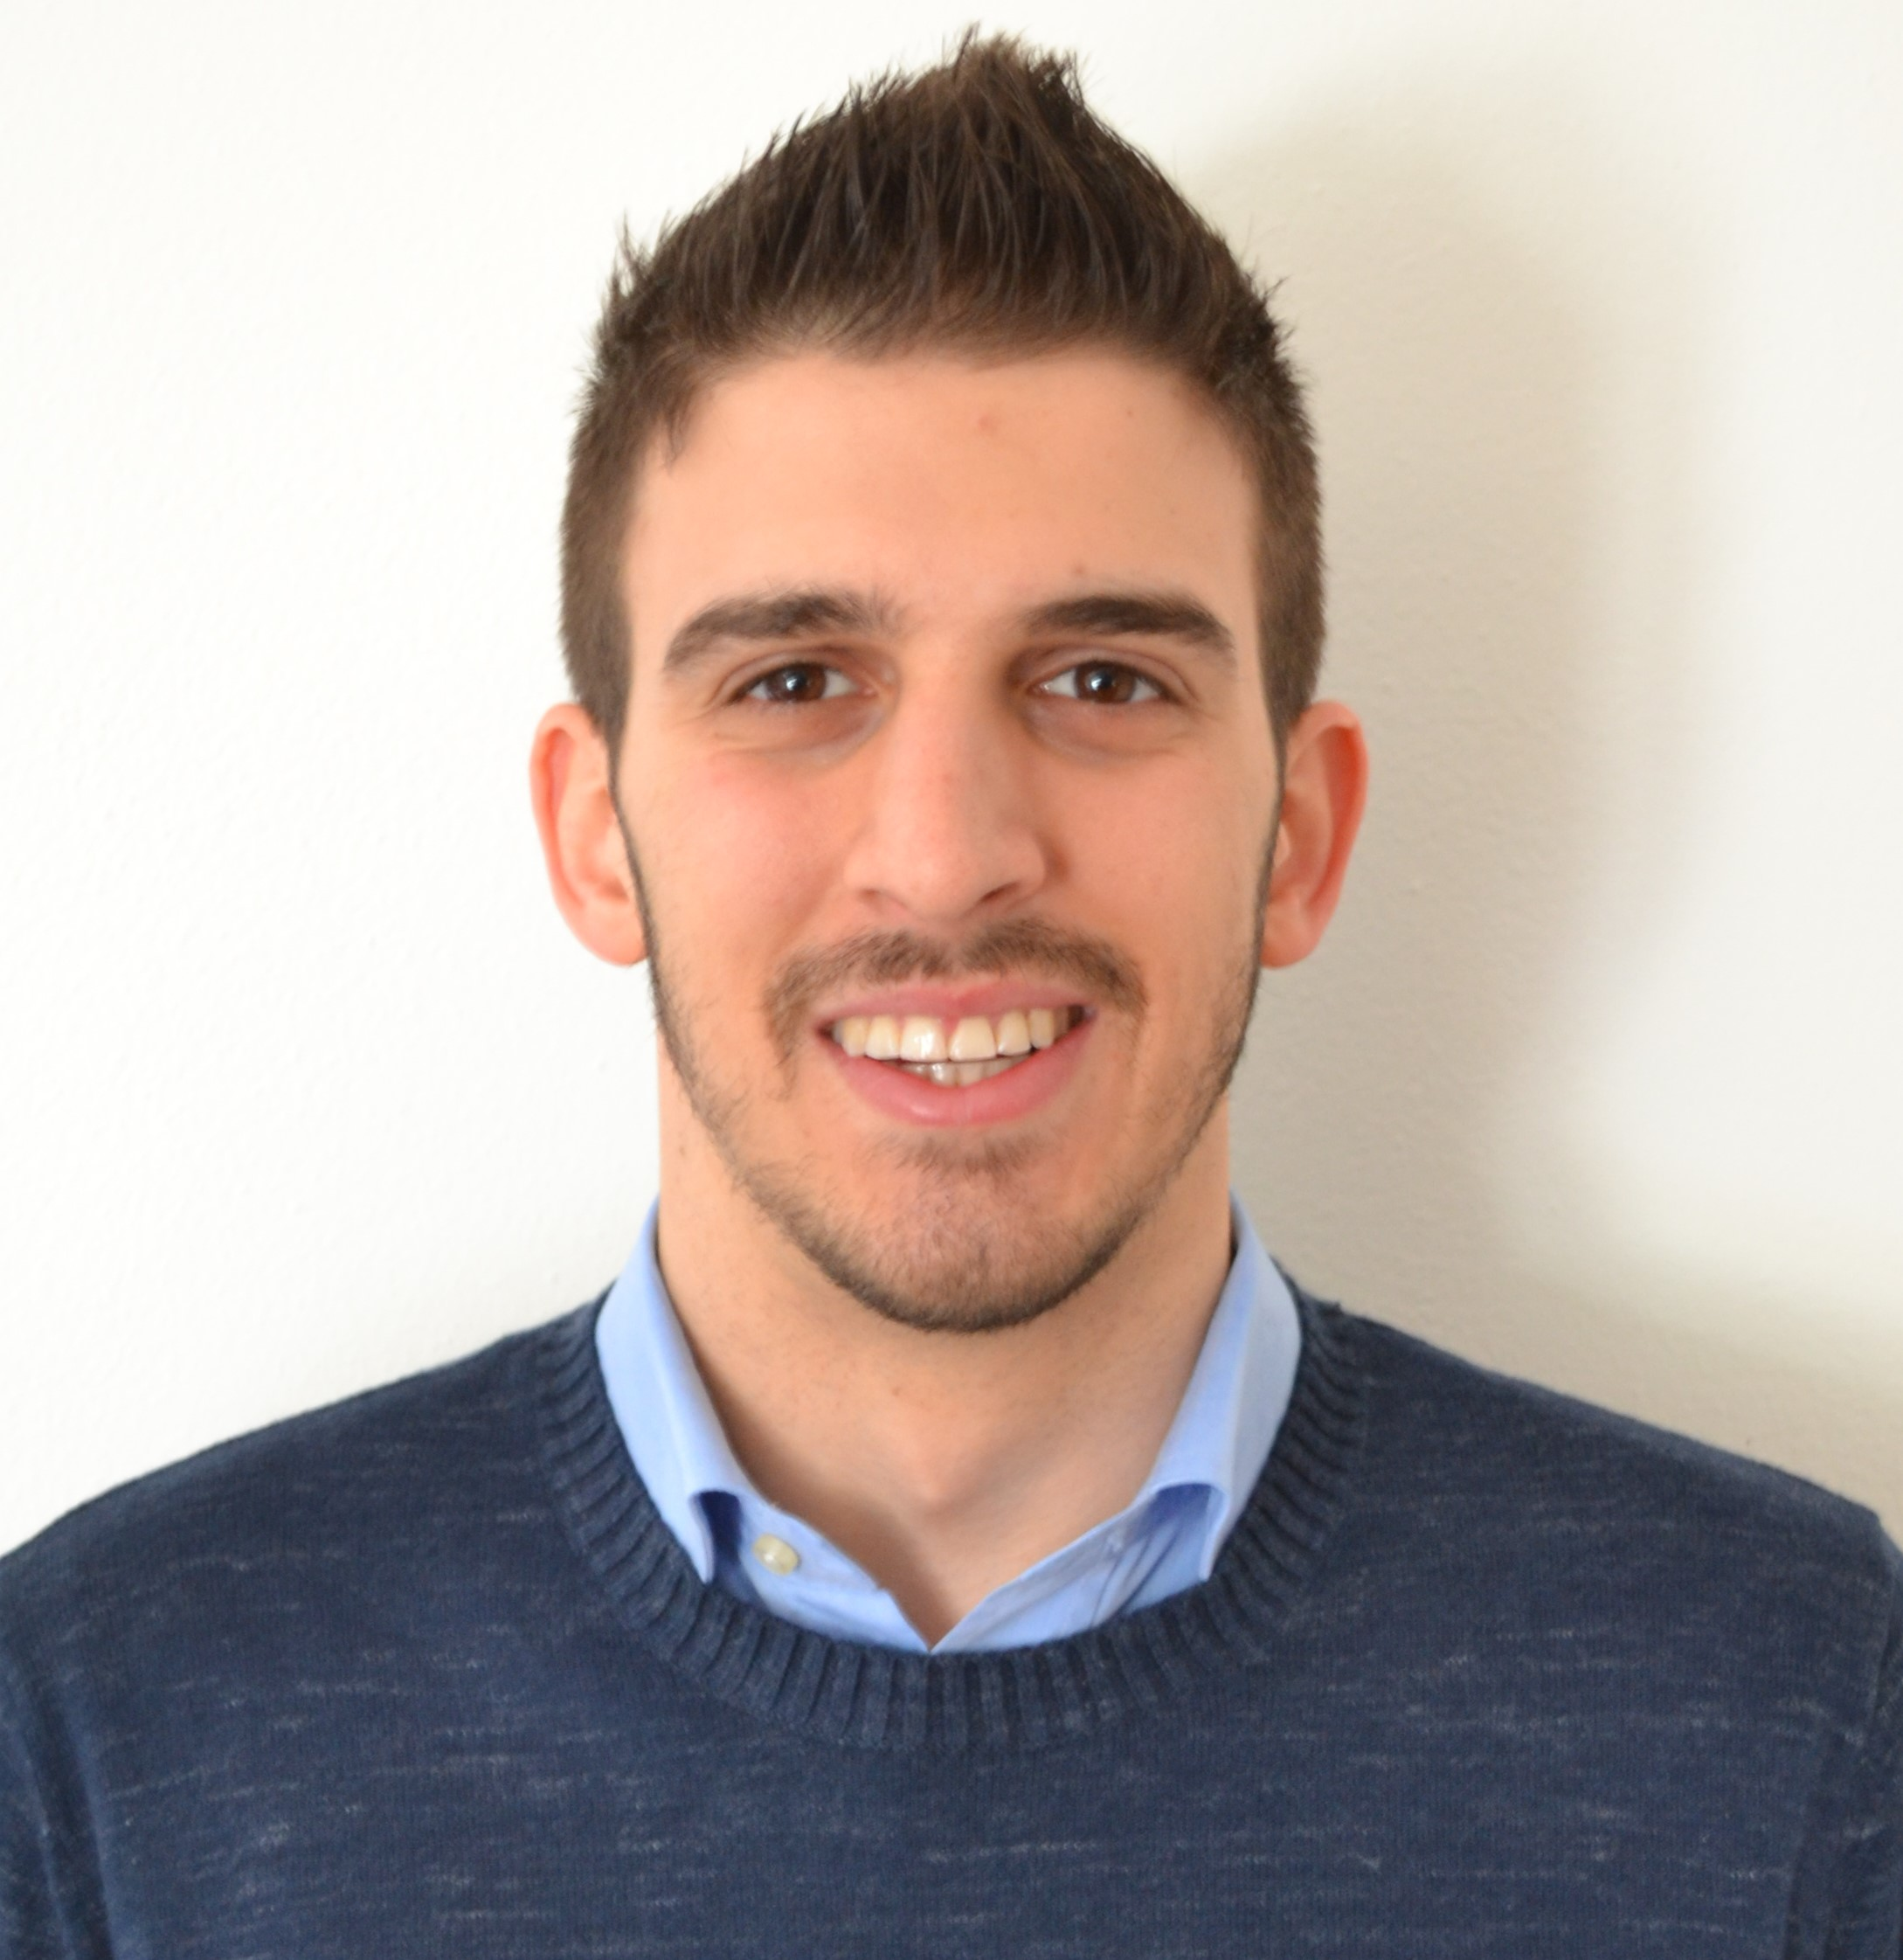
\includegraphics[width=1.0\linewidth]{Fototessera.jpg}
\end{minipage}
%
% \vspace{0.5cm}
%	INTRODUCTION, SKILLS AND TECHNOLOGIES
%
\cvsect{Chi sono?}
%
\begin{minipage}[t]{0.5\textwidth} % 40% of the page width for the introduction text
	\vspace{-\baselineskip} % Required for vertically aligning minipages
Sono un laureato in ingegneria meccatronica a cui piacciono le sfide e mettersi in gioco alla continua ricerca di occasioni di crescita professionale e personale.
Sono una persona molto determinata che non ha paura uscire dalla sua zona di comfort per ottenere i risultati richiesti. Sono curioso, non mi fermo all'apparenza e cerco di dare il massimo ed ottimizzare tutto ciò che faccio.
Professionalmente sono esperto di modellistica e controllo di sistemi meccatronici con particolare focus sul controllo ottimo.
%
\end{minipage}
\hfill % Whitespace between
\begin{minipage}[t]{0.45\textwidth} % 50% of the page for the skills bar chart
	\vspace{-\baselineskip} % Required for vertically aligning minipages
	\begin{barchart}{5.5}
		\baritem{Maple}{100}
		\baritem{Matlab}{80}
		\baritem{C/C++}{60}
		\baritem{LaTeX}{70}
		\baritem{Python}{80}
		\baritem{Ruby}{40}
	\end{barchart}
\end{minipage}
%
% \begin{center}
% 	\bubbles{5/Inventor,3/AutoCAD, 4/ANSYS,3/Visual Studio}
% \end{center}
%
%	EXPERIENCE
%

\cvsect{Esperienze lavorative}
%
\begin{entrylist}
	\entry
		{Sett. 2021-In corso}
		{Assistente alla didattica}
		{Università di Trento}
		{Assistente alla didattica per il corso di Sistemi Meccanici e Modelli. Docente: Prof. Mauro Da Lio.}
	\entry
		{Gen. 2021-In corso}
		{Assegno di ricerca (Decreto n. 205/2020)}
		{Università di Trento}
		{Titolo: “Confronto algoritmi di risoluzione di problemi controllo ottimo di tempo minimo per veicoli da competizione". \\
		Supervisore: Prof. Francesco Biral.}
	\entry
		{Giu.-Dic.2020}
		{Borsa di studio per attività di ricerca (Decreto n. 74/2020)}
		{Università di Trento}
		{Titolo: “Manovre di tempo minimo di modelli di veicoli complessi descritti con DAE".\\
		Supervisore: Prof. Francesco Biral.}
	\entry
		{Apr. -Giu. 2019 \&\\Sett.-Dic. 2019 \&\\Sett.-Dic. 2018}
		{Video-lezioni e Tutorato aree specifiche meccanica e meccatronica}
		{Università di Trento}
		{Lezioni, dispense ed esercizi in inglese per studenti del CdL magistrale in ingegneria meccatronica. Video-lezioni realizzate per il dipartimento di ingegneria industriale.\\
		Supervisori: Prof. Francesco Biral, Prof. Enrico Bertolazzi e Prof. Daniele Fontanelli}
	\entry
		{Giu.-Sett. 2017\\\footnotesize{Tirocinio}}
		{Tirocinante reparto controllo qualità}
		{SIAP s.p.a. gruppo CARRARO}
		{Misure di precisione di componenti meccanici, redazione carte sequenziali, piani di controllo specifici, CCP, misure per studi di capacità (Cp e Cpk).
		}
	% \entry
	% 	{Giu.--Sett. 2013 \&\\Giu.--Sett. 2012}
	% 	{Apprendista idraulico }
	% 	{DE NARDO ALESSANDRO IMPIANTI TERMOIDRAULICI}
	% 	{Apprendista idraulico durante la stagione estiva.}
\end{entrylist}
%
%	EDUCATION
%
\cvsect{Educazione}
%
\begin{entrylist}
	\entry
		{Dic. 2020}
		{Abilitazione professionale all'esercizio della professione di Ingegnere}{Università di Trento}{Ingegnere Industriale}
	\entry
		{2017 -- 2020}
		{Laurea Magistrale in Ingegneria Meccatronica}
		{Università di Trento}
		{Curriculum meccanica e meccatronica. Laurea magistrale in lingua inglese.\\
		Corsi principali: modellazione e simulazione di sistemi meccatronici, dinamica e controllo di veicoli e robot, progettazione meccanica, controlli automatici.
		\hfill Voto:108/110} 
		% \textit{computer vision}, vibrazioni meccaniche, , controlli automatici , robotica industriale
	\entry
		{2013 -- 2017}
		{Laurea Triennale in Ingegneria Meccanica}
		{Università degli studi di Udine}
		{Corsi principali: termodinamica e trasmissione del calore,  macchine a fluido, meccanica dei solidi, costruzione di macchine, tecnologia meccanica.} %\hfill Voto:94/110
	% \entry
	% 	{2008 -- 2013}
	% 	{Diploma di liceo scientifico}
	% 	{Liceo Scientifico "Michelangelo Grigoletti"}
	% 	{Diploma di liceo scientifico con indirizzo PNI (piano nazionale informatica). } % \hfill Voto:67/100
\end{entrylist}
%
%	ADDITIONAL INFORMATION
%
\begin{minipage}[t]{0.3\textwidth}
	\vspace{-\baselineskip} % Required for vertically aligning minipages
	\cvsect{Lingue}
%
	\textbf{Italiano} - Madrelingua\\
	\textbf{Inglese}  - Fluente, livello C1 (IELTS)
%
\end{minipage}
\hfill
\begin{minipage}[t]{0.3\textwidth}
	\vspace{-\baselineskip} % Required for vertically aligning minipages
	%
	\cvsect{Hobbies}
	%
	% Sono appassionato di IoT, tecnologia e smart gadget.
	% Creo progetti attuati automaticamente con Arduino e Raspberry Pi.
	Sono appassionato di tecnologia a tutto tondo. Dalle fotocamere ai computer di nuova generazione.
%
	% Sono un appassionato della montagna a $360$ gradi e mi piace cimentarmi in lavori di \textit{bricolage} ed altri fai-da-te più tecnologici con Arduino e Raspberry Pi.
%
\end{minipage}
\hfill
\begin{minipage}[t]{0.3\textwidth}
	\vspace{-\baselineskip} % Required for vertically aligning minipages
	%
	\cvsect{Sports}
%
	% Sono un arrampicatore sportivo amatoriale ed un disceto sciatore.
	Pratico attivamente arrampicata sportiva, sci alpino, scialpinismo, corsa.
%
\end{minipage}

\hfill
% \hline
% Maniago, \today
% \hline
\pagebreak

%----------------------------------------------------------------------------------------

\cvsect{Privacy}

Autorizzo il trattamento dei dati personali contenuti nel mio curriculum vitae in base all’art. 13 del D. Lgs. 196/2003 e all’art. 13 del Regolamento UE 2016/679 relativo alla protezione delle persone fisiche con riguardo al trattamento dei dati personali.

\vspace{0.5cm}
Maniago, \today \\

\vspace{0.2cm}

\includegraphics[width=0.25\textwidth]{firma.jpg}


\end{document}
